\documentclass[10pt,a4paper,twocolumn,twoside]{article}
\usepackage[utf8]{inputenc}
\usepackage[catalan]{babel}
\usepackage{multicol}
\usepackage{graphicx}
\usepackage{fancyhdr}
\usepackage{times}
\usepackage{titlesec}
\usepackage{multirow}
\usepackage{lettrine}
\usepackage[top=2cm, bottom=1.5cm, left=2cm, right=2cm]{geometry}
\usepackage[figurename=Fig.,tablename=TAULA]{caption}
\usepackage{hyperref}
\usepackage[ampersand]{easylist}

\captionsetup[table]{textfont=sc}


\graphicspath{{img/}}
\ListProperties(Progressive*=0.5cm)

\author{\normalsize\sffamily Kevin Martín Fernández}
\title{\huge{\sffamily Simulation environment to capture images from drone}}
\date{}

\newcommand\blfootnote[1]{%
  \begingroup
  \renewcommand\thefootnote{}\footnote{#1}%
  \addtocounter{footnote}{-1}%
  \endgroup
}

%
%\large\bfseries\sffamily
\titleformat{\section}
{\large\sffamily\scshape\bfseries}
{\textbf{\thesection}}{1em}{}

\begin{document}

\fancyhead[LO]{\scriptsize Kevin Martín: Simulation environment to capture images from drone}
\fancyhead[RO]{\thepage}
\fancyhead[LE]{\thepage}
\fancyhead[RE]{\scriptsize EE/UAB TFG INFORMÀTICA: Simulation environment to capture images from drone}

\fancyfoot[CO,CE]{}

\fancypagestyle{primerapagina}
{
   \fancyhf{}
   \fancyhead[L]{\scriptsize TFG EN ENGINYERIA INFORMÀTICA, ESCOLA D'ENGINYERIA (EE), UNIVERSITAT AUTÒNOMA DE BARCELONA (UAB)}
   \fancyfoot[C]{\scriptsize ``Mes'' de 2019, Escola d'Enginyeria (UAB)}
}

%\lhead{\thepage}
%\chead{}
%\rhead{\tiny EE/UAB TFG INFORMÀTICA: TÍTOL (ABREUJAT SI ÉS MOLT LLARG)}
%\lhead{ EE/UAB \thepage}
%\lfoot{}
%\cfoot{\tiny{February 2015, Escola d'Enginyeria (UAB)}}
%\rfoot{}
\renewcommand{\headrulewidth}{0pt}
\renewcommand{\footrulewidth}{0pt}
\pagestyle{fancy}

%\thispagestyle{myheadings}
\twocolumn[\begin{@twocolumnfalse}

{
\vspace*{-1cm}
\maketitle
}

\thispagestyle{primerapagina}
%\twocolumn[\begin{@twocolumnfalse}
%\maketitle
%\begin{abstract}
\begin{center}
\parbox{0.915\textwidth}
{\sffamily\small
\textbf{Abstract--} Resum
\\
\\
\textbf{Keywords-- }
Simulator, Drone, Terrain, Satellite, Multi-spectral, Unreal Engine\\
\\
%\end{abstract}
}

\bigskip

{\vrule depth 0pt height 0.5pt width 4cm\hspace{7.5pt}%
\raisebox{-3.5pt}{\fontfamily{pzd}\fontencoding{U}\fontseries{m}\fontshape{n}\fontsize{11}{12}\selectfont\char70}%
\hspace{7.5pt}\vrule depth 0pt height 0.5pt width 4cm\relax}

\end{center}

\bigskip
%\end{abstract}
\end{@twocolumnfalse}]

\blfootnote{$\bullet$ E-mail de contacte: kevinmf94@gmail.com}
\blfootnote{$\bullet$ Menció realitzada: Enginyeria de Computació}
\blfootnote{$\bullet$ Treball tutoritzat per: Felipe Lumbreras Ruíz}
\blfootnote{$\bullet$ Curs 2018/19}

\vspace{-1cm}
\section{Introducció}

\lettrine[lines=2]{L}{a} simulació de espais per a la generació de imatges artificials és un àmbit en el que es busca representa el mon real de la forma més realista possible per tal de poder generar informació que en entorns reals ens representaria un perill o un cost econòmic elevat, d'aquesta forma es pot arribar a ensenyar als algoritmes d'aprenentatge reduint la quantitat d'informació real que es necessitaria.\\
En aquest treball és vol aconseguir que mitjançant dades obtingudes a traves de càmeres de diferents mitjans aeris com poden ser satèl·lits, avions o drons podem representar terreny real en entorns simulats.

\section{Objectius}

En aquest apartat determinarem els diferents objectius del projecte en format de jerarquia per tal de veure la dependència entre els diferents objectius:

\begin{easylist}
& Analitzar
&& Investigar l'estat de l'art
&&& Investigar entorn AirSim
&&& Investigar entorn Carla
&& Definir els objectius
&& Estudiar el entorn Unreal Engine
&& Investigar els mapes d'altura
&& Investigar les imatges tant RGB com multi-espectrals
&& Investigar webservices WMS
&& Investigar llibreries RCP
& Definir
&& Definir mòduls interessants pel projecte
&& Definir l'estructura del software
&&& Definir els mòduls a desenvolupar
&&& Definir la comunicació entre els mòduls
&&& Definir estructura de les dades que rebrà Unreal Engine
& Desenvolupar
&& Desenvolupar modul de transformació i obtenció de dades
&&& Desenvolupar el modul de transformació de dades d'altura i textures
&&& Desenvolupar l'importador de dades en Unreal Engine
&& Desenvolupar modul gràfic (Ureal Engine)
&&& Desenvolupar la interfície del menú
&&& Desenvolupar el mòdul per importar fitxers personalitzats en Unreal Engine
&&& Desenvolupar codi per la generació del terreny
&&& Desenvolupar codi per la generació dels materials
&&&& Visualitzar diferents materials (RGB, Multiespectre, etc)
&&& Desenvolupar codi  de servidor per control del vehicle
&& Desenvolupar modul de scripting
&&& Desenvolupament client que controlara el vehicle
&& Integrar els mòduls de AirSim en Unreal Engine
&&& Integrar modul de Drons en el projecte
&&& Integrar modul de Segmentació en el projecte
&& Desenvolupar altres capes d'informació
& Testejar
&& Fer provàs del modul de transformació de dades
&&& Provar amb dades locals
&&& Provar amb dades externes
&& Fer provàs del modul gràfic 
&& Fer provàs del modul de control per scripting
&&& Elaborar script d'exemple
&&& Provar script d'exemple
& Documentar
&& Redactar informe inicial
&& Redactar informe de seguiment I
&& Redactar informe de seguiment II
&& Redactar el informe final
&& Elaborar proposta de presentació
&& Elaborar pòster

\end{easylist}

\section{Estat de l'art}

Actualment existeixen diverses aplicacions per la generació d'imatges en entorns que simulen la realitat amb la finalitat de generar dades per algoritmes d'aprenentatge.
En aquest àmbit unes de les més importants és AirSim \cite{airsim} desenvolupat per Microsoft sobre el motor gràfic Unreal Engine aquest entorn permet la simulació de cotxes i drons, control per scripts, simulació climatològica, simulació del sol, generació d'imatges en visualització com son rgb, segmentació o profunditat, etc... Per altra banda un altre entorn similar al anterior és Carla \cite{carla} aquest software esta enfocat en cotxes ja que el seu principal objectiu es obtenir dades per l'aprenentatge de cotxes autònoms.

\begin{figure}[!h]
\centering
  	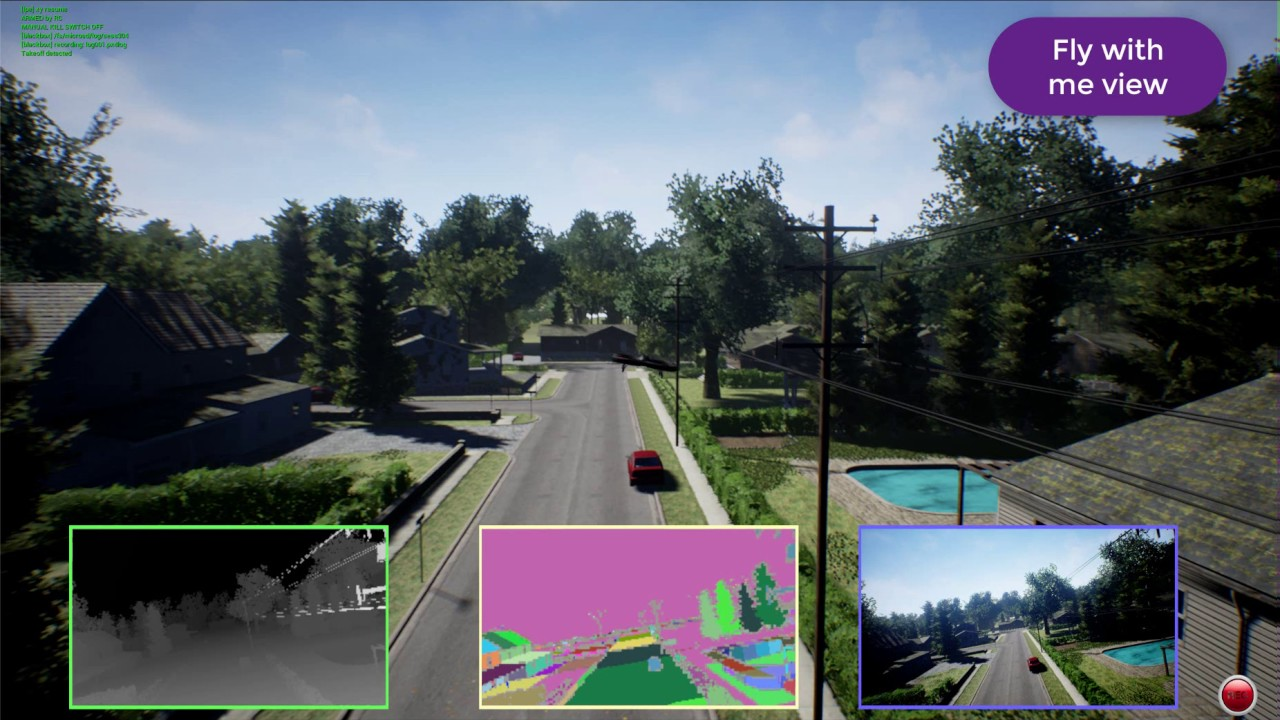
\includegraphics[width=0.4\textwidth]{airsim}
	\caption{Simulador Airsim}
	\label{fig-airsim}
\end{figure}

\section{Metodologia}

En aquest projecte hem decidit utilitzar una metodologies de tipus Agile \cite{agile} ja que això ens permetrà identificar de una forma millor les petites parts de les que es composa aquest projecte, a més a més d'adaptar-se als canvis imprevistos. En concret s'ha escollit la tècnica Kanban \cite{kanban} que consisteix en organitza el nostre backlog (tasques de curta duració) en 
targetes que ficarem en un taulell segons en quin punt del cicle de vida de la tasca es trobi (pendent, començada, etc) per això s'ha decidit utilitzar l'eina Trello \cite{trello} que permet de forma visual crear targetes i moure-les entre les diferents llistes.

\subsection{Diagrama de Gant}

\section{Projecte}

\section{Conclusions}


\section*{Agraïments}


\begin{thebibliography}{11}
\bibitem{airsim}
AirSim - \url{https://github.com/Microsoft/AirSim} [19/02/2019]


\bibitem{carla}
Carla - \url{http://carla.org} [19/02/2019]

\bibitem{agile}
Agile software development
\\ \url{https://en.wikipedia.org/wiki/Agile_software_development}
[19/02/2019]

\bibitem{kanban}
Kanban
\\ \url{https://www.iebschool.com/blog/metodologia-kanban-agile-scrum/} [19/02/2019]

\bibitem{trello}
Trello - \url{https://trello.com/} [19/02/2019]


\end{thebibliography}

\appendix

\section*{Apèndix}

\setcounter{section}{1}

\subsection{Secció d'Apèndix}
\subsection{Secció d'Apèndix}
\subsection{Secció d'Apèndix}



\end{document}

